\section{Results}
	Following the development of the RAG system, including data ingestion, chunking, embedding, and retrieval-generation components, the next step involves evaluating the system’s performance. The evaluation focuses on the effectiveness of different chunking and embedding strategies, the quality of retrieved context, and the fidelity of generated responses. The results presented below summarize the outcomes of these experiments, highlighting system behavior across multiple configurations.
	
\subsection{Scraping Ablation}
To evaluate ingestion performance, two scraping pipelines were compared: Playwright and Puppeteer. Both were applied on the same set of JioPay business and help center pages, with metrics recorded for the number of pages processed, total tokens extracted, proportion of noisy text, throughput, and failure rates.

Playwright was tested for its robustness in handling dynamic content and its ability to extract both text and images.

Puppeteer was tested for its coverage of documents, particularly in capturing PDFs, despite requiring multiple runs in certain cases.

The results are summarized in Table 1, providing a quantitative basis for analyzing trade-offs in completeness, robustness, and efficiency between the two scraping approaches.

\begin{table}[h!]
	\centering
	\caption{Comparison of Playwright and Puppeteer Scraping Results}
	\label{tab:scraping_results}
	\begin{tabular}{|l|c|c|}
		\hline
		\textbf{Metric}       & \textbf{Playwright} & \textbf{Puppeteer} \\ \hline
		Pages (Raw)           & 28                  & 28                 \\ \hline
		Pages (Cleaned)       & 25                  & 25                 \\ \hline
		Tokens (Raw)          & 563,620             & 563,085            \\ \hline
		Tokens (Cleaned)      & 36,282              & 36,282             \\ \hline
		Noise (\%)            & 93.56               & 93.56              \\ \hline
		Throughput (tokens/page) & 1451.28           & 1451.28            \\ \hline
		Failures (\%)         & 0.00*               & 0.00*              \\ \hline
	\end{tabular}
	\\[1ex]
	\footnotesize{* Failures not reflected in cleaned dataset; Puppeteer required 2–3 retries and occasional manual reloads.}
\end{table}

\begin{itemize}
	\item Playwright successfully completed the scraping in a single run, demonstrating greater robustness against dynamic loading delays.
	
	\item Puppeteer often required 2–3 execution attempts for the same dataset. Failures occurred when sites took longer to load, causing Puppeteer to prematurely close the browser. In some cases, manual reloading was required to complete the scrape.
	
	\item In terms of data quality, both frameworks produced nearly identical cleaned datasets. The noise reduction was significant (93.5\%), indicating that cleaning effectively filtered out irrelevant boilerplate content.
	
	\item Throughput was consistent across both tools at around 1450 tokens per page, reflecting stable processing efficiency once data was successfully extracted.
	
	\item The failure rate was effectively zero in the cleaned dataset, but observationally, Puppeteer exhibited higher practical failures due to retries and manual intervention.
	
	\item PDF Extraction: Puppeteer was more effective at capturing PDFs, managing to fetch nearly all of them, while Playwright failed to consistently scrape embedded PDF resources.
\end{itemize}

\subsection{Chunking Ablation}
	
The evaluation employed a unified, multi-dimensional framework designed to balance domain-specific content quality with retrieval effectiveness, size optimization, and performance benchmarking. This approach integrates two complementary paradigms: domain-specific RAG quality assessment, which emphasizes semantic accuracy and contextual adequacy of retrieved content, and retrieval performance evaluation, which focuses on the effectiveness of retrieval in answering task-specific queries.

A weighted scoring system was adopted to aggregate results across dimensions. Content quality and domain relevance (RAG Quality) contributed 45\% to the overall score, retrieval effectiveness metrics accounted for 40\%, chunk size optimization contributed 8\%, and processing efficiency and latency comprised the remaining 7\%. This balance ensured that strategies were judged not only on retrieval accuracy but also on the adequacy, compactness, and efficiency of their outputs.

RAG quality assessment was operationalized through five metric groups. Semantic coherence was evaluated by detecting broken or fragmented sentences, measuring topic consistency against JioPay domain-specific keywords, and assessing completeness of thought in Q\&A and procedural content. Context completeness was examined across content types, with standards tailored to FAQs (Q\&A pair integrity), PDF documents (section completeness within 30–200+ word thresholds), and web content (contextual adequacy by word count). Information density was quantified through keyword presence, numerical detail, procedural instruction coverage, and normalized density scores. Topic coverage analysis measured cross-category balance across JioPay domains, including payments, app usage, business, support, and features. Finally, FAQ grouping quality was assessed based on clustering coherence, ensuring related queries and answers were grouped appropriately within domain contexts.

Retrieval performance metrics followed standard information retrieval practices, including Precision@1 for top-ranked relevance, Precision@K and Recall@K for coverage and breadth, and Mean Reciprocal Rank (MRR) for evaluating the ranking position of the first relevant result. Chunk size optimization was guided by a framework defining an optimal range of 80–400 tokens and an acceptable range of 50–600 tokens, with graduated penalties applied for deviations. Performance benchmarking captured query processing latency (mean and tail latencies), throughput in queries per second, and normalized scores to enable fair comparison.

The test dataset comprised fifteen comprehensive queries reflecting real-world JioPay usage across five categories—onboarding, payments, KYC, API/security, pricing, and features. Queries were stratified by complexity into simple, medium, and complex cases, with ground truth topic mappings defined for relevance validation.

The evaluation process followed a structured flow: data loading and normalization across chunking formats, statistical analysis of token and character distributions, domain-specific quality assessment using the five RAG dimensions, retrieval simulation with TF-IDF similarity, performance benchmarking, and final weighted score aggregation. Comparative analysis across strategies was conducted to produce multi-strategy rankings.

Results were reported through a structured framework comprising an executive summary highlighting the best-performing strategies, detailed rankings with weighted scores, per-strategy metric breakdowns, and category-level analyses by query type. Multi-dimensional radar charts and other visualizations were employed to provide interpretable comparisons, and deployment readiness metadata was generated to assess production applicability.

\begin{table*}[htbp]
	\centering
	\caption{Chunk Size Analysis Across Different Strategies}
	\resizebox{\textwidth}{!}{
		\begin{tabular}{lccccccc}
			\hline
			\textbf{Strategy} & \textbf{Total Chunks} & \textbf{Min Tokens} & \textbf{Max Tokens} & \textbf{Avg Tokens} & \textbf{Median Tokens} & \textbf{Std Tokens} \\
			\hline
			Fixed\_256\_0             & 642  & 1     & 258    & 219.9 & 256.0 & 74.4 \\
			Fixed\_512\_64            & 415  & 17    & 514    & 382.8 & 512.0 & 193.7 \\
			Fixed\_1024\_128          & 262  & 17    & 1025   & 599.0 & 958.0 & 449.8 \\
			Semantic\_High\_Sim       & 1486 & 6     & 833    & 93.3  & 72.0  & 80.3 \\
			Semantic\_Low\_Sim        & 1065 & 8     & 833    & 130.2 & 84.0  & 127.5 \\
			Semantic\_Med\_Sim        & 1320 & 6     & 833    & 105.1 & 77.0  & 91.5 \\
			Structural\_Balanced      & 368  & 3     & 1499   & 235.1 & 69.5  & 387.6 \\
			Structural\_Hierarchical  & 380  & 3     & 1197   & 227.7 & 72.0  & 341.1 \\
			Structural\_Large         & 489  & 1     & 13693  & 175.8 & 32.0  & 740.2 \\
			Recursive\_Balanced       & 619  & 1     & 1018   & 158.3 & 61.0  & 200.6 \\
			Recursive\_Large          & 600  & 1     & 1258   & 163.3 & 59.5  & 227.7 \\
			Recursive\_Small          & 654  & 1     & 758    & 150.0 & 69.5  & 171.1 \\
			LLM\_smallChunks          & 584  & 14    & 16627  & 107.1 & 52.0  & 898.6 \\
			\hline
		\end{tabular}
	}
\end{table*}

\begin{table*}[htbp]
	\centering
	\caption{Unified Chunking Strategy - Content and Retrieval Metrics}
	\resizebox{\textwidth}{!}{
		\begin{tabular}{lcccccccccc}
			\hline
			\textbf{Strategy} & \textbf{Semantic Coh} & \textbf{Context Comp} & \textbf{Info Density} & \textbf{Topic Cov} & \textbf{Precision@1} & \textbf{Recall@5} & \textbf{MRR} & \textbf{Latency (ms)} & \textbf{QPS} \\
			\hline
			Fixed\_256\_0         & 0.252 & 0.859 & 0.454 & 1.000 & 0.733 & 0.944 & 0.856 & 54.49 & 18.4 \\
			Fixed\_512\_64        & 0.242 & 0.847 & 0.446 & 1.000 & 0.800 & 0.928 & 0.872 & 75.09 & 13.3 \\
			Fixed\_1024\_128      & 0.277 & 0.827 & 0.441 & 1.000 & 0.800 & 0.906 & 0.883 & 63.13 & 15.8 \\
			Semantic\_High\_Sim   & 0.459 & 0.707 & 0.420 & 1.000 & 0.667 & 0.944 & 0.811 & 71.83 & 13.9 \\
			Semantic\_Low\_Sim    & 0.429 & 0.735 & 0.412 & 1.000 & 0.667 & 0.939 & 0.811 & 68.95 & 14.5 \\
			Semantic\_Med\_Sim    & 0.448 & 0.722 & 0.418 & 1.000 & 0.733 & 0.922 & 0.856 & 66.98 & 14.9 \\
			Structural\_Balanced  & 0.356 & 0.720 & 0.608 & 1.000 & 0.867 & 0.967 & 0.922 & 63.68 & 15.7 \\
			Structural\_Hierarchical & 0.348 & 0.726 & 0.606 & 1.000 & 0.867 & 0.967 & 0.922 & 68.97 & 14.5 \\
			Structural\_Large     & 0.413 & 0.624 & 0.595 & 1.000 & 0.867 & 0.944 & 0.933 & 63.46 & 15.8 \\
			Recursive\_Balanced   & 0.348 & 0.700 & 0.619 & 1.000 & 0.800 & 0.939 & 0.900 & 62.47 & 16.0 \\
			Recursive\_Large      & 0.350 & 0.694 & 0.628 & 1.000 & 0.800 & 0.939 & 0.900 & 63.57 & 15.7 \\
			Recursive\_Small      & 0.348 & 0.710 & 0.614 & 1.000 & 0.800 & 0.939 & 0.900 & 55.67 & 18.0 \\
			LLM\_smallChunks      & 0.477 & 0.702 & 0.542 & 1.000 & 0.867 & 0.967 & 0.933 & 36.83 & 27.1 \\
			\hline
		\end{tabular}
	}
\end{table*}


\begin{table*}[htbp]
	\centering
	\caption{Unified Chunking Strategy - Core Metrics}
	\begin{tabular}{lccccc}
		\hline
		\textbf{Strategy} & \textbf{Final Score} & \textbf{RAG Quality} & \textbf{Retrieval Perf} & \textbf{Size Opt} & \textbf{Performance} \\
		\hline
		Fixed\_256\_0         & 0.704 & 0.641 & 0.843 & 0.970 & 0.003 \\
		Fixed\_512\_64        & 0.695 & 0.634 & 0.860 & 0.826 & 0.002 \\
		Fixed\_1024\_128      & 0.686 & 0.636 & 0.854 & 0.722 & 0.003 \\
		Semantic\_High\_Sim   & 0.680 & 0.647 & 0.799 & 0.866 & 0.002 \\
		Semantic\_Low\_Sim    & 0.681 & 0.644 & 0.801 & 0.880 & 0.002 \\
		Semantic\_Med\_Sim    & 0.692 & 0.647 & 0.828 & 0.875 & 0.002 \\
		Structural\_Balanced  & 0.724 & 0.671 & 0.902 & 0.758 & 0.002 \\
		Structural\_Hierarchical & 0.725 & 0.670 & 0.906 & 0.766 & 0.002 \\
		Structural\_Large     & 0.710 & 0.658 & 0.889 & 0.723 & 0.002 \\
		Recursive\_Balanced   & 0.706 & 0.666 & 0.856 & 0.787 & 0.003 \\
		Recursive\_Large      & 0.706 & 0.668 & 0.856 & 0.784 & 0.002 \\
		Recursive\_Small      & 0.709 & 0.668 & 0.856 & 0.814 & 0.003 \\
		LLM\_smallChunks      & 0.742 & 0.680 & 0.925 & 0.815 & 0.007 \\
		\hline
	\end{tabular}
\end{table*}


Although the unified evaluation identified LLM\_smallChunks as the top-performing strategy (Final Score 0.742, RAG Quality 0.680, Retrieval Performance 0.925), practical considerations regarding chunk sizes rendered it less suitable for deployment. Consequently, the next best-performing strategies, Structural\_Hierarchical (Final Score 0.725) and Structural\_Balanced (Final Score 0.724), were selected for implementation. These strategies offer a balanced trade-off between retrieval effectiveness, semantic coherence, and manageable chunk sizes, making them more appropriate for real-world deployment scenarios.


	\begin{figure}[htbp]
		\centering
		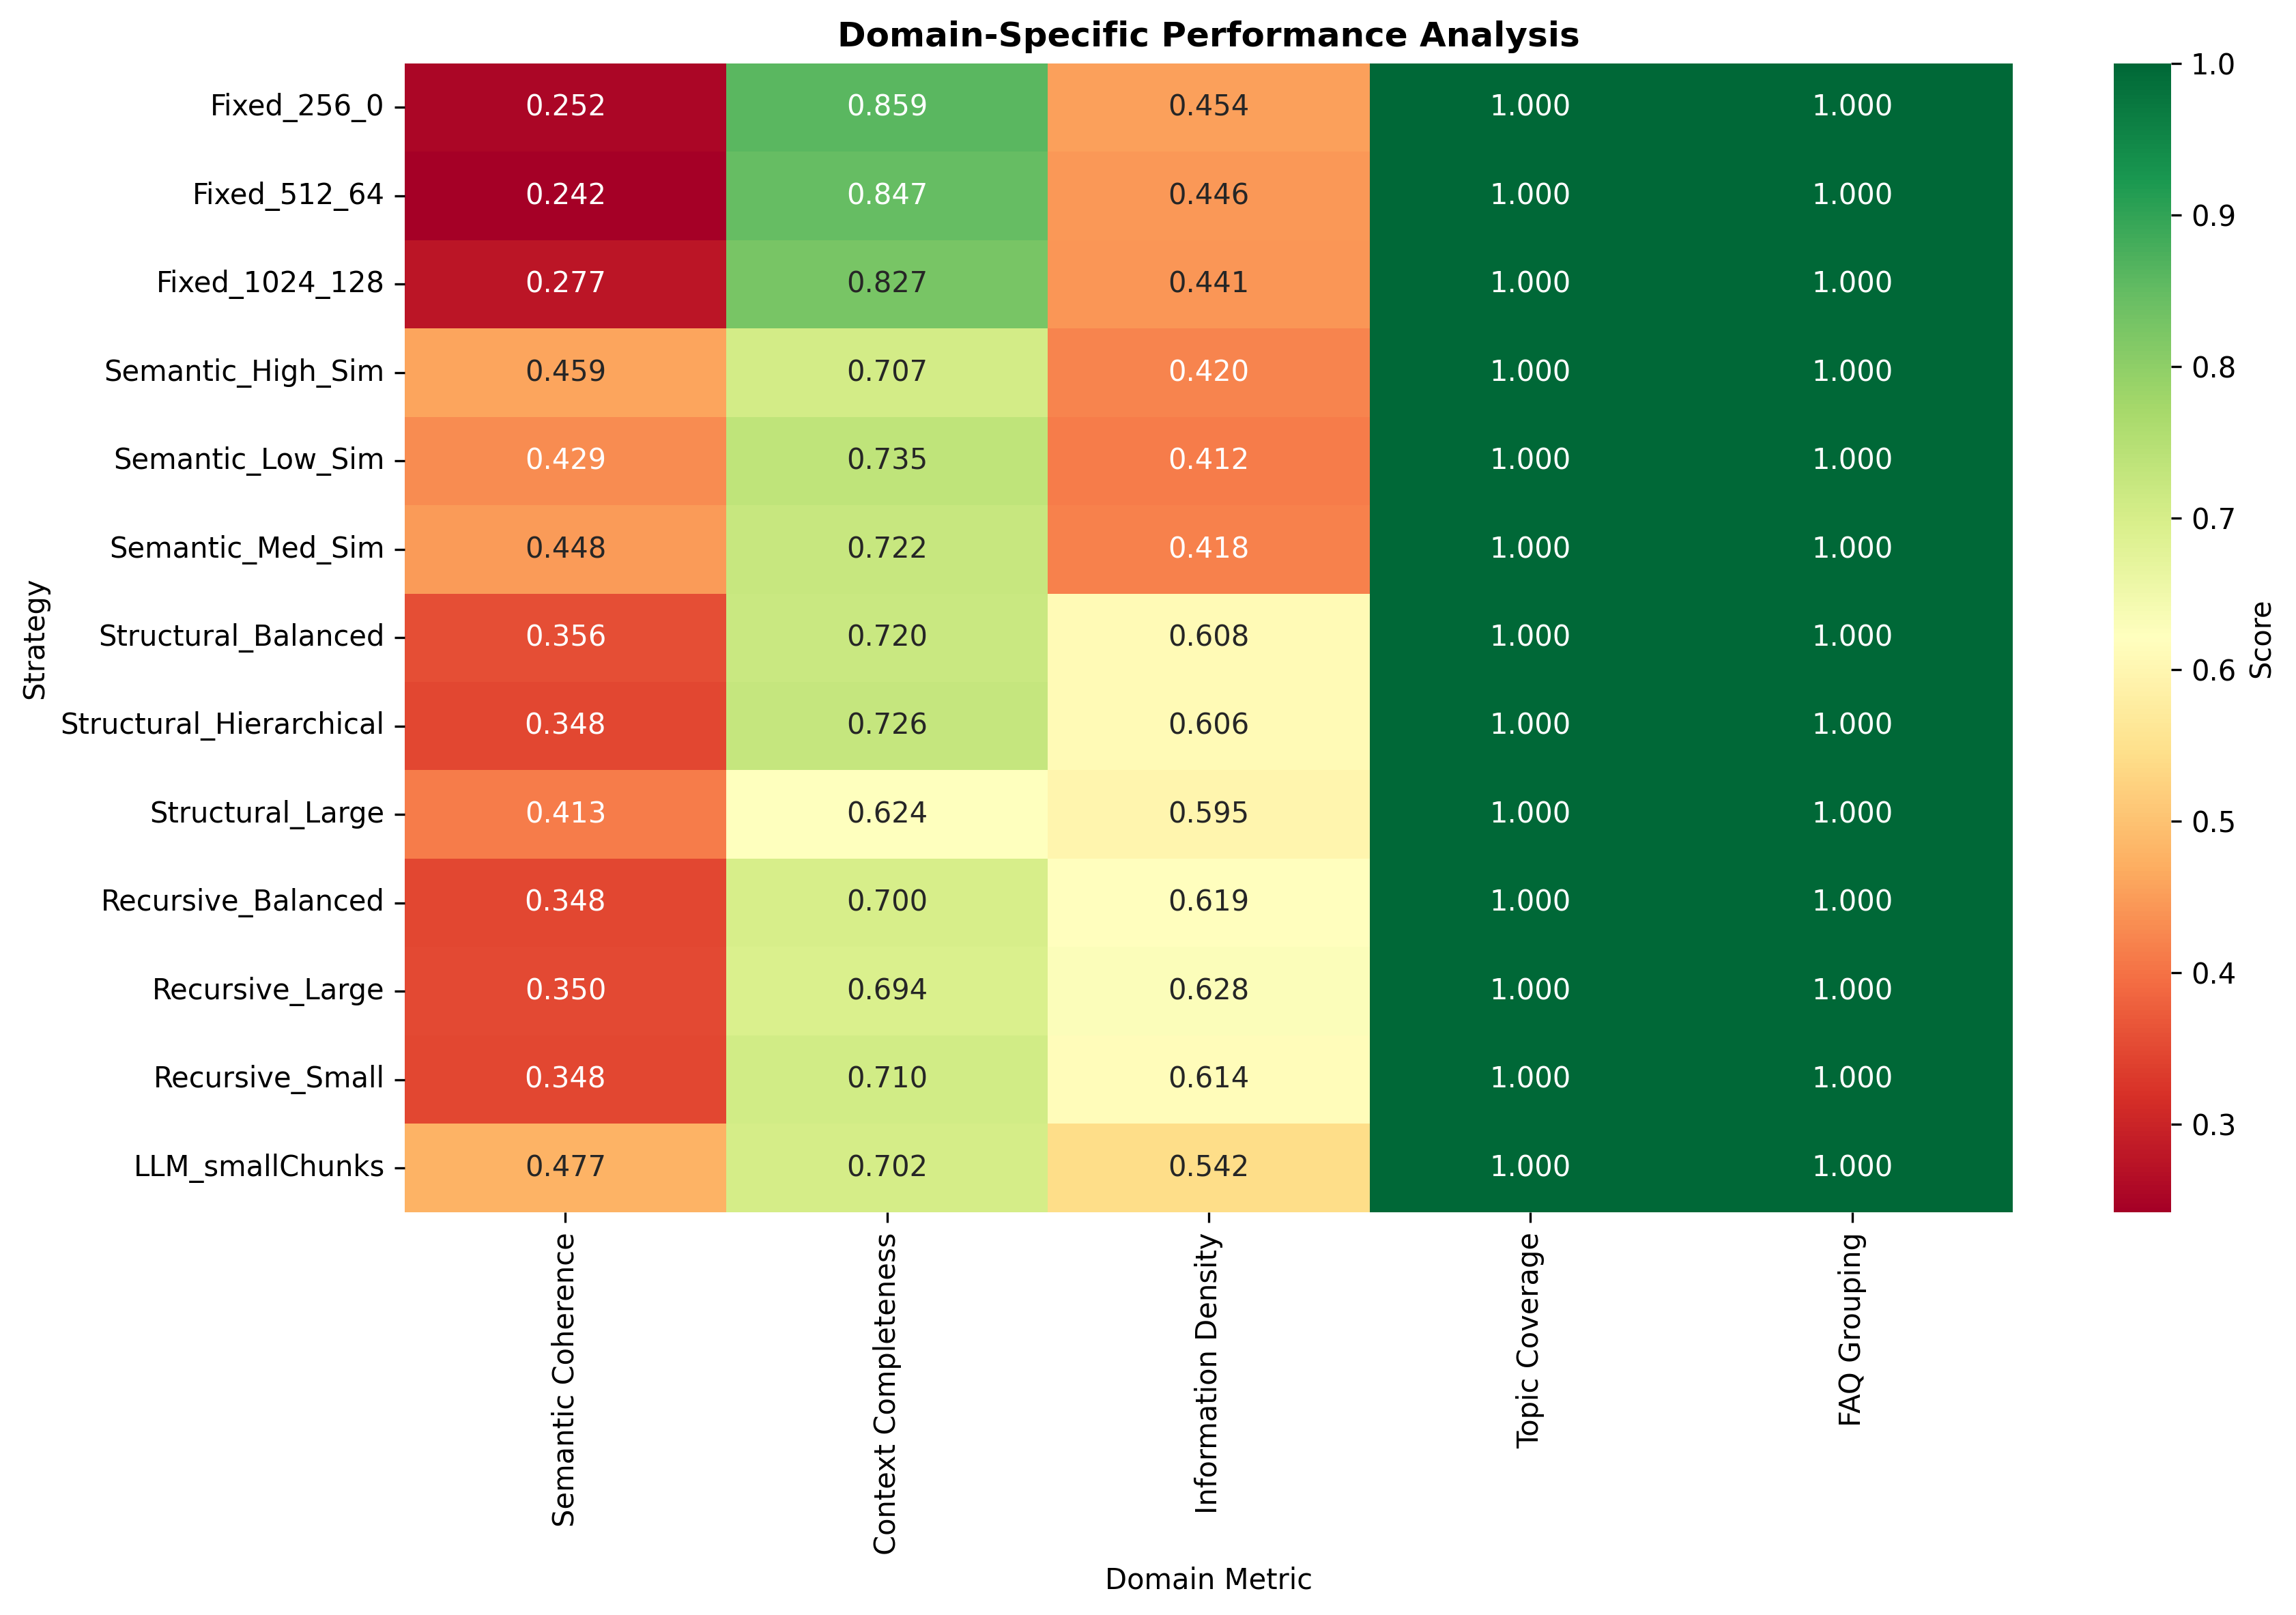
\includegraphics[width=0.6\linewidth,keepaspectratio]{domain_performance_heatmap.png}
		\caption{Domain Wise Performance Heatmap}
		\label{fig1}
	\end{figure}
	
	\begin{figure}[htbp]
		\centering
		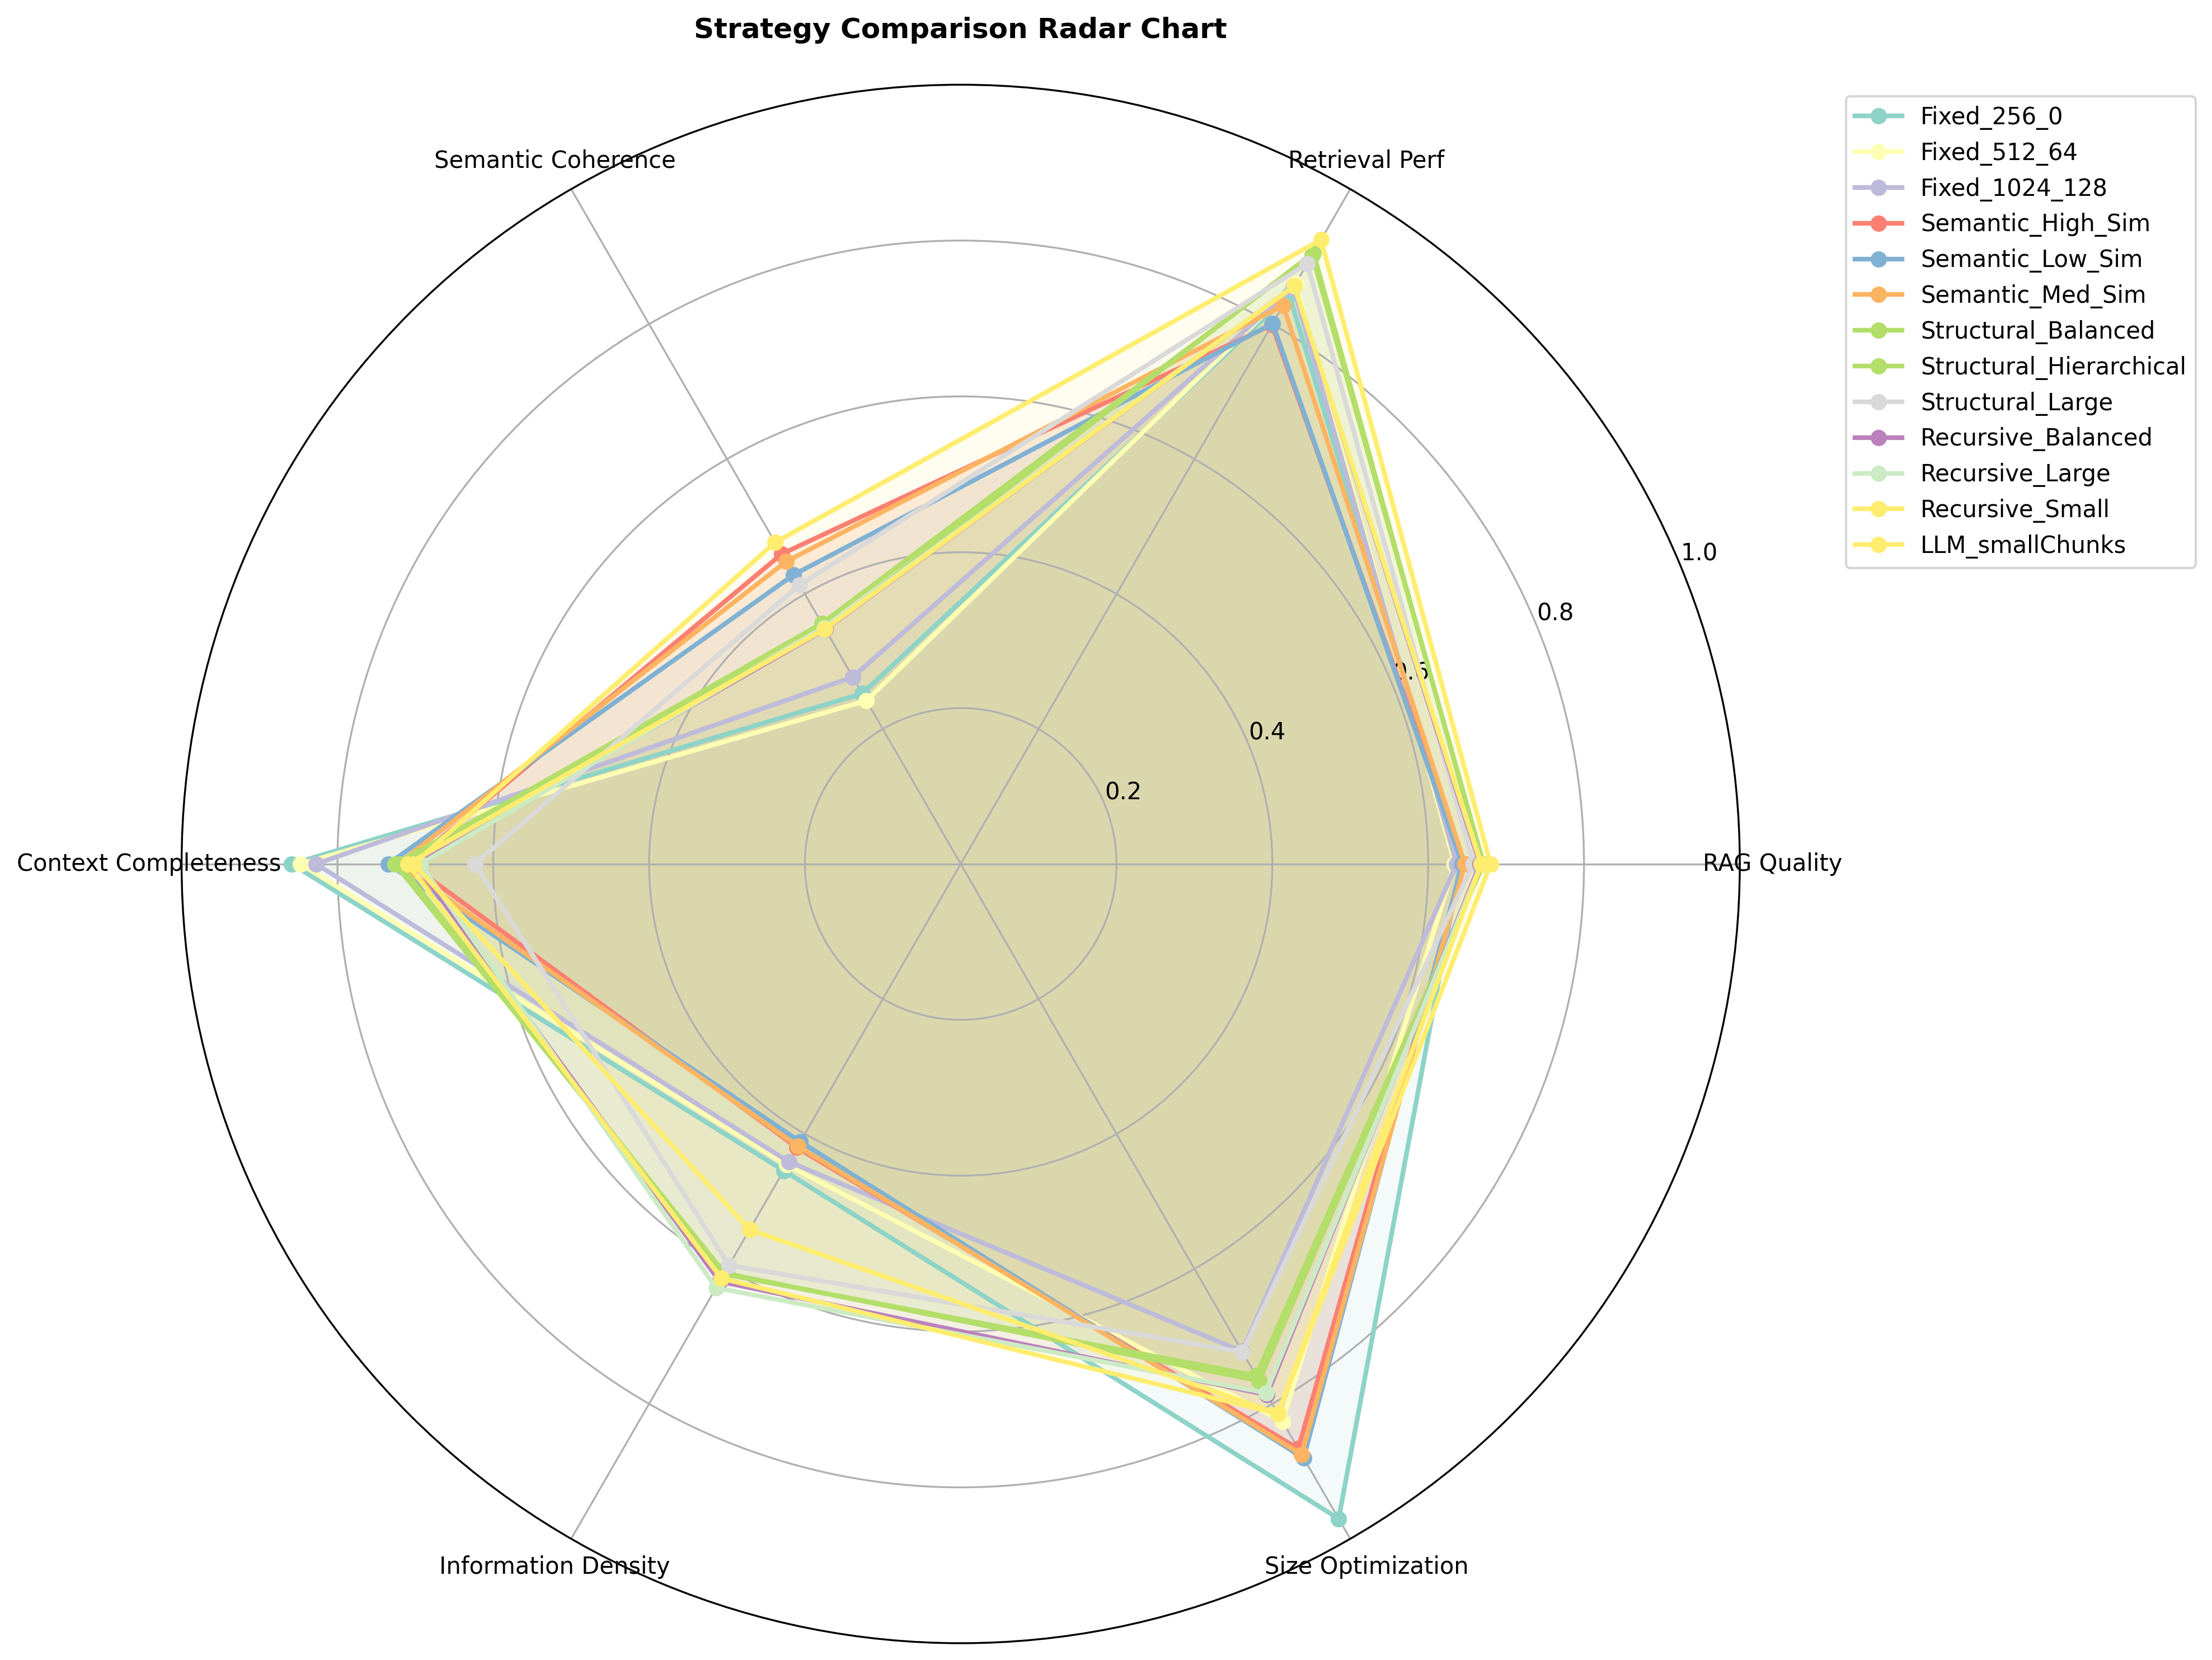
\includegraphics[width=0.6\linewidth,keepaspectratio]{strategy_radar_chart.png}
		\caption{Strategy Radar Chart}
		\label{fig2}
	\end{figure}
	
	\begin{figure}[htbp]
		\centering
		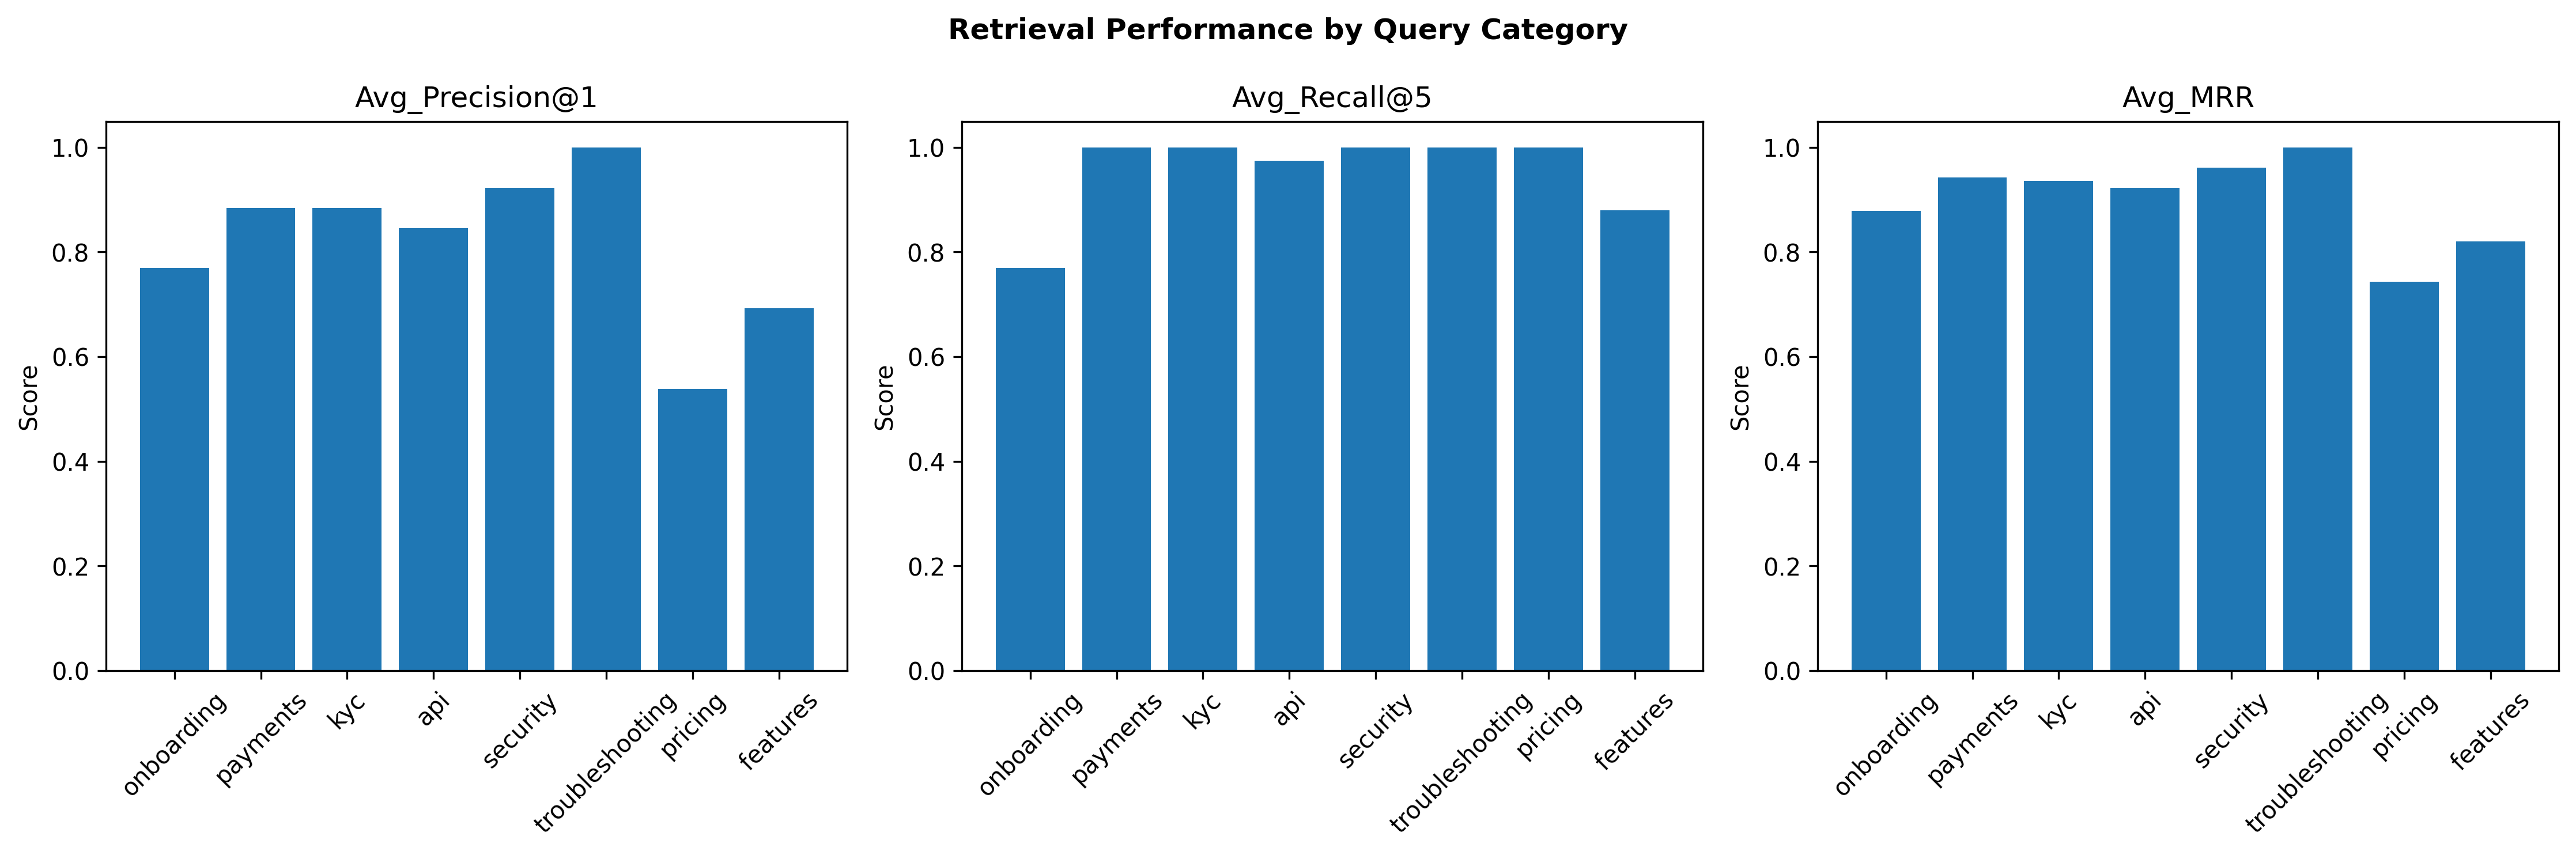
\includegraphics[width=0.6\linewidth,keepaspectratio]{retrieval_by_category.png}
		\caption{Retrieval by Category Metrics}
		\label{fig3}
	\end{figure}
	
	\begin{figure}[htbp]
		\centering
		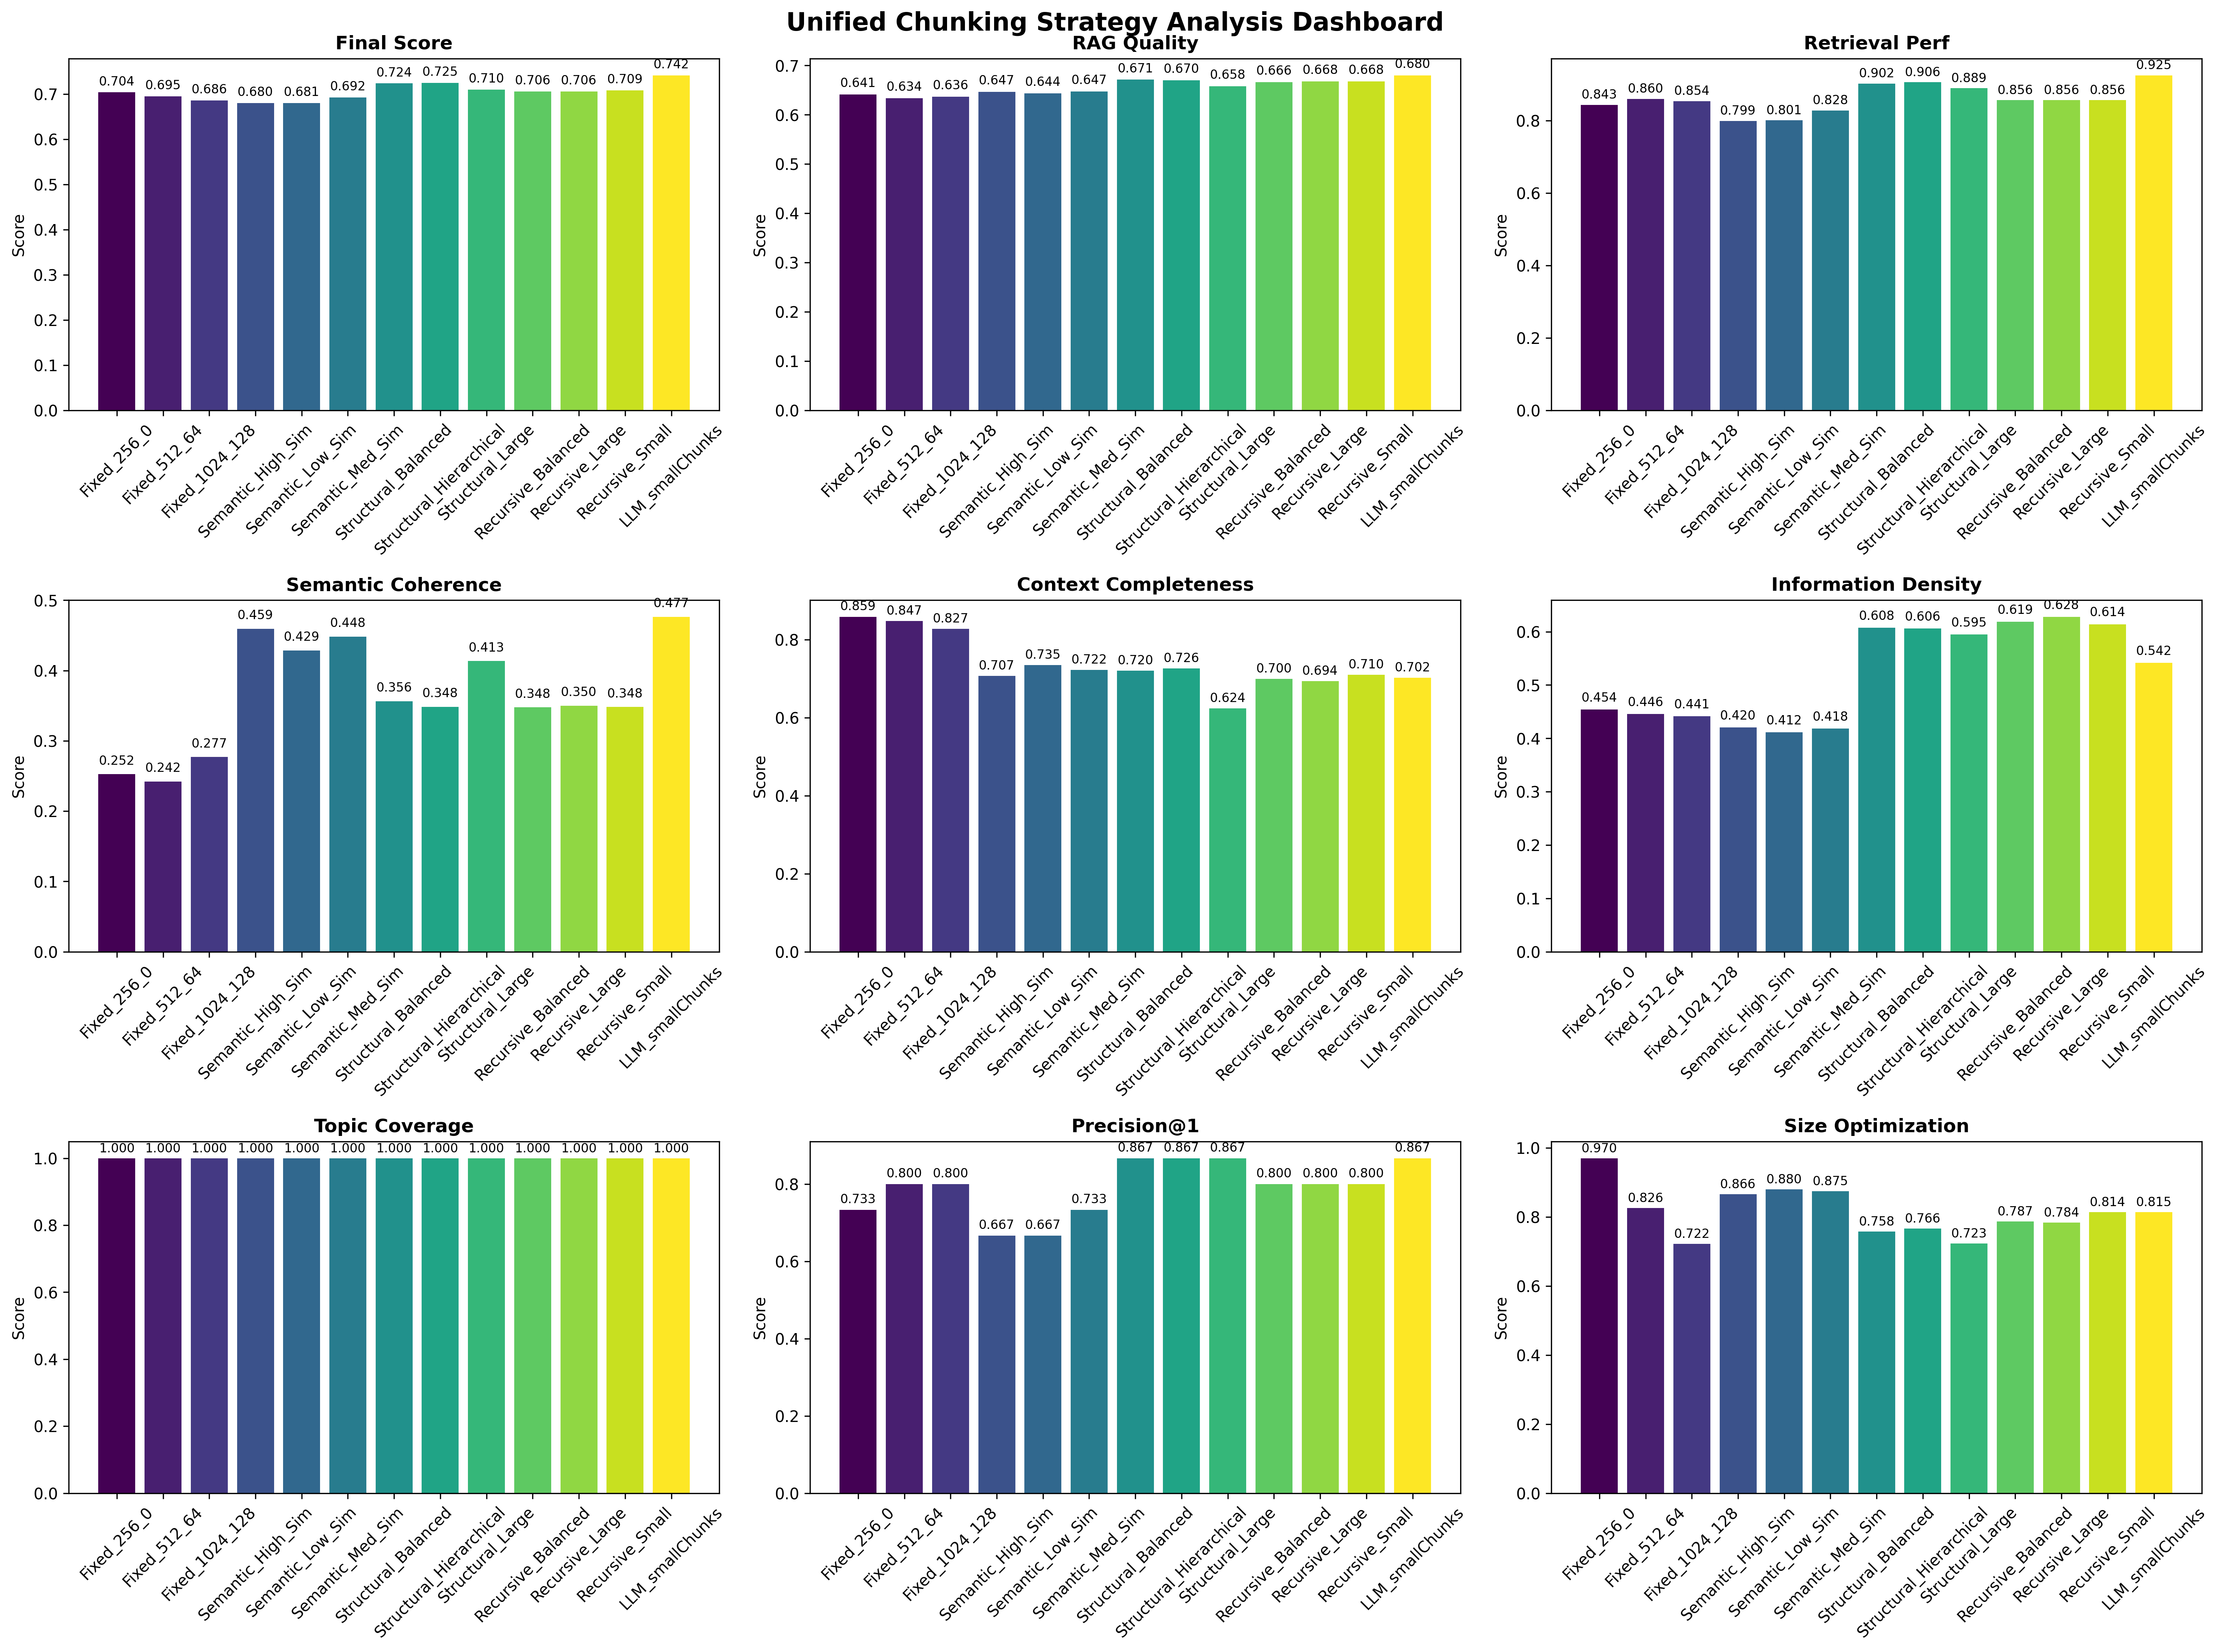
\includegraphics[width=0.6\linewidth,keepaspectratio]{unified_performance_dashboard.png}
		\caption{Unified Metrics Graphs}
		\label{fig4}
	\end{figure}
	
	\subsection{Embedding Evaluation}
	Following the selection of Structural Balanced and Structural Hierarchical as the most viable chunking strategies, three embedding models were evaluated: Qwen3 0.6B (1024 dimensions), Google EmbeddingGemma-300M (768 dimensions), and Voyage-3.5 (1024 dimensions). The evaluation considered retrieval quality (recall@5, mean reciprocal rank, precision@5) as well as efficiency (index size, average latency, and success rate). The embedding models were chosen from HuggingFace's MTEB leaderboard for their high retrieval accuracy.
	
	The embedding evaluation was conducted by applying each model to the outputs of the two selected chunking strategies (Structural Hierarchical and Structural Balanced). The embeddings generated by each model were indexed, and retrieval performance was assessed using a standardized query set.
	
	Performance was measured across multiple metrics, including Recall@5, Precision@1, Mean Reciprocal Rank (MRR), and Success Rate, alongside efficiency indicators such as average query latency and queries per second (QPS). In addition, index size was recorded to assess storage overhead.
	
	All experiments were executed within a unified framework, ensuring consistency in preprocessing, indexing, and benchmarking. The results were consolidated into comparative tables to facilitate a fair evaluation of each embedding model’s effectiveness and efficiency.
	
\begin{table*}[htbp]
	\centering
	\caption{Embedding Model Evaluation on Structural Balanced and Structural Hierarchical Strategies}
	\resizebox{\textwidth}{!}{%
		\begin{tabular}{lccccccc}
			\hline
			\textbf{Strategy} & \textbf{Model} & \textbf{Recall@5} & \textbf{MRR} & \textbf{Precision@5} & \textbf{Index Size (MB)} & \textbf{Latency (ms)} & \textbf{Success Rate (\%)} \\
			\hline
			\multirow{3}{*}{Structural Balanced} 
			& Qwen3-0.6B & 0.396 & 0.367 & 0.347 & 420 & 119.6 & 83.3 \\
			& Gemma-300M & 0.271 & 0.379 & 0.271 & 315 & 50.8  & 91.7 \\
			& Voyage-3.5 & 0.958 & 0.903 & 0.883 & 512 & 18900 & 66.7 \\
			\hline
			\multirow{3}{*}{Structural Hierarchical} 
			& Qwen3-0.6B & 0.354 & 0.337 & 0.319 & 422 & 120.1 & 83.3 \\
			& Gemma-300M & 0.250 & 0.360 & 0.250 & 317 & 52.3  & 91.7 \\
			& Voyage-3.5 & 0.958 & 0.901 & 0.875 & 514 & 19020 & 66.7 \\
			\hline
	\end{tabular}}
\end{table*}
	
	
	Across both chunking strategies, Voyage-3.5 consistently achieved the strongest retrieval effectiveness, though at the cost of significantly higher latency, rendering it impractical for real-time deployments. Qwen3 0.6B provided a balanced trade-off between accuracy and efficiency, while EmbeddingGemma-300M emphasized speed and reliability, albeit with lower retrieval quality. This contrast highlights the trade-offs between retrieval strength and computational efficiency in practical embedding model selection.
	
	\subsection{RAG Evaluation}
	The final evaluation stage integrated both retrieval and generation. Queries were retrieved, reranked, and passed to the language model with guardrails applied. The generated responses were then directly compared against ground-truth answers scraped from the source knowledge base.
	
	This evaluation measured answer quality, retrieval effectiveness, and system performance. The consolidated results are presented in Table~\ref{tab:rag_results}.
	
	\begin{table}[htbp]
		\centering
		\caption{Final RAG Evaluation Results with Answer Quality, Retrieval, and System Performance Metrics}
		\label{tab:rag_results}
		\begin{tabular}{lcc}
			\hline
			\textbf{Category} & \textbf{Metric} & \textbf{Value} \\
			\hline
			\multirow{6}{*}{Answer Quality} 
			& Overall Quality Grade & A (0.715) \\
			& Semantic Similarity   & 0.756 \\
			& Faithfulness          & 0.680 \\
			& Completeness          & 0.717 \\
			& Relevance             & 0.677 \\
			& Exact Match           & 0.469 \\
			\hline
			\multirow{5}{*}{Grade Distribution} 
			& A & 55.0\% \\
			& B & 40.0\% \\
			& C & 0.0\% \\
			& D & 5.0\% \\
			& F & 0.0\% \\
			\hline
			\multirow{4}{*}{Retrieval} 
			& Similarity Score    & 0.756 \\
			& Threshold Pass Rate & 95.0\% \\
			& Precision@1         & 0.743 \\
			& Mean Reciprocal Rank & 0.756 \\
			\hline
			\multirow{5}{*}{System Performance} 
			& Latency (Mean)  & 2863 ms \\
			& Latency (P50)   & 2769 ms \\
			& Latency (P95)   & 3480 ms \\
			& Memory Usage    & 404.7 MB \\
			& CPU Usage       & 20.3\% \\
			\hline
		\end{tabular}
	\end{table}
	
	